% Thesis template by Aleksander M. Stensby
% aleksander.stensby@gmail.com

\documentclass[12pt,letterpaper,final]{report}
%\documentclass[12pt,a4paper,final]{report}
\usepackage{makeidx}
\usepackage{varioref}
\usepackage{setspace}
\usepackage{times} % Use this package for times-font. %%not found
\usepackage{fancyvrb}
\usepackage{moreverb}
\usepackage{fancyhdr}
\usepackage{epsfig}
\usepackage{eucal}
\usepackage{amsmath}
\usepackage{amsfonts}
\usepackage{floatflt}
\usepackage{tocbibind}
\usepackage{wrapfig}
\usepackage{listings}
\usepackage{color}
\usepackage{amsthm}
\usepackage{subfigure}
\usepackage{longtable}
\usepackage{url}
\usepackage{multicol}
\usepackage{array}
\usepackage[style=list,toc=true]{glossaries}
\usepackage{graphicx} %For � kunne inkludere grafikk
\usepackage{hiafrontpage} % For UoA Style frontpage.
\usepackage{rotating}

\definecolor{Brown}{cmyk}{0,0.81,1,0.60}
\definecolor{OliveGreen}{cmyk}{0.64,0,0.95,0.40}
\definecolor{Keyword}{cmyk}{0.66,0.90,0.33,0.20}
\definecolor{Comment}{cmyk}{0.88,0.35,1.00,0.30}
\definecolor{Identifier}{cmyk}{1,1,1,1}
\definecolor{XmlKeyword}{cmyk}{0.66,0.90,0.33,0.20}
\definecolor{FrameColor}{cmyk}{0.66,0.90,0.33,0.20}
\definecolor{XmlIdentifier}{cmyk}{0,0.81,1,0.60}
\definecolor{XmlString}{cmyk}{1,1,1,1}


%%%% Fancy
% 11pt font
%\headheight=13.6 pt

% 12pt font
\headheight=14.5 pt

\pagestyle{fancy} 
\fancyhead[L]{\leftmark}
\fancyhead[R]{}
%lowercase
%\renewcommand{\chaptermark}[1]{\markboth{#1}{}}

%Fit more figures on a page
\renewcommand{\topfraction}{.99}
\renewcommand{\bottomfraction}{.99}
\renewcommand{\textfraction}{.01}
\renewcommand{\floatpagefraction}{.99}

% spacing:
%\singlespacing
\onehalfspacing
%\doublespacing

\theoremstyle{definition}
\newtheorem{theorem}{Theorem}
\hyphenation{theorem}
\newtheorem{definition}{Definition}
\newtheorem{remark}{Remark}

\oddsidemargin=0.5in \evensidemargin=0.3in
\parskip=0.0 true in

\author{Haakon Bakkevig Steinsholt and Daniel Aasen}
\titlelogo{images/uia_logo_large} %Path to UoA logo.
\title{Route for Safe Evacuation of Passengers in Crises Situations}

\draftversion{0.1}
%\date{January 9, 2007} %specify own date

\makeglossary

%for draft work, select the chapters to include in the pdf but still keep all cross-references intact.
%\includeonly{introduction}

\begin{document}

    \maketitle

    \newpage    
    %\begin{abstract}
Your absctract goes here. 
Thesis template by Aleksander M. Stensby.
\end{abstract}

    %\chapter*{Preface}

Your preface goes here.

    \tableofcontents
    \listoffigures
    %\listoftables

    \parskip=0.1 true in

    \newpage

		% General structure, normally (background, and solution chapter may be split into several different chapters!
    \chapter{Introduction}
\label{ch:introduction}

\section{Background}

Pathfinding algorithms are used to find the quickest path between two points. 
These algorithms are for instance used to solve mazes, scheduling a long trip in
metro systems or wire routing. In our project we have looked at using pathfinding
algorithms to find the safest route off a ship that is on fire.

Every year people die in boating accidents and we hope that our work can be
used to save lives. Jim Hall, the Chairman of the National Transportation 
Safety Board testified in front of the Subcommittee on Coast Guard and Maritime 
Transportation, making several safety recomendations after the Scandinavian Star
accident \cite{ntsb}. One of them were to "Improve crew language/communication 
ability to assist passengers during emergencies." Our work, which will be part of a system
that provides passengers with the quickest route to the exit, could output 
any directions in the language of the phone owner. This would not only improve 
communication if the employees and passengers do not speak the same language, 
it would also ensure that the directives reach all passengers quicker than if the employees 
were to guide all passengers. Additionally it increases the probability that all passengers 
receives proper guidance. For instance any message played over a sound system could be
difficult to hear during a panic and passengers could be in rooms or corridors
where they would be unrachable for the employees.

\section{Problem Statement}

Morten Goodwin from the University of Agder proposed a project about finding a safe route
to evacuate passengers in crisis situations. As there are a multitude of pathfinding algorithms
we chose to focus on exploring the validity of a single algorithm called Ant Colony Optimization 
(ACO). We chose this algorithm since we believed the nature of the algorithm made it a perfect
candidate in a dynamic environment. Our goal was to create a testing environment in which 
we would run the ACO algorithm and then evaluate its performance.

To reach the project goal within the deadline some limitations were set. Firstly, the simulations did not use 
any real data. Secondly, the graphs were completely randomly generated and the graphs did not resemble
any ships or their actual structure. Thirdly, all rooms were equally easy to traverse and had unlimited capasity. 
Finally, there were no efforts to simulate actual human behavior during a crisis and all passengers followed
any directions perfectly.

Additionally we made several assumptions. Firstly, we asumed that a ship could be sufficently modeled
as a graph. Secondly, everyone on the ship had access to a smart phone with an application that ran our
algorithms and they followed the directions perfectly. Finally, all passengers acted the same and moved at
the same speed.

\section{Solution Approach}

Normally, pathfinding algorithms finds the quickest path from a location to an 
exit. However in our case certain sections of the ship could be dangerous and the algorithms 
had to find alternate routes, valuing safety over speed. The ships were modeled as undirected
graphs with nodes and vertices. The nodes represented any type of room, including
hallways, stairs etc., and a vertex between two nodes indicated that it was possible to
cross over from one to the other.

ACO attempts to find the optimal route through the ship by mimicking the behavior of ants and ant colonies. 
The performance of the algorithm was tested by creating random graphs with a specific amount of
passengers in them. We would then run ACO multiple times and compare its performance against
random behavior and perfect behavior. In the case of random behavior the passengers would randomly
walk until they either died or found the exit. And to simulate perfect behavior we found every possible
path for every passenger and chose the best one.

\section{Report outline}

Chapter one gives an overview of how pathfinding algorithms work, what problem we are ting to solve with our
project and our approach to doing so. Additionally it explains our motivation for doing it as well as sets some
limitations and assumptions to the process. The second chapter contains the state of the art which we drew
knowledge from to complete our project. ACO is described in detail, both by showing the formulas and describing
the ideas that lead to the creation of the algorithm.

    
    \chapter{State of the art}
\label{ch:background}

\section{Ant Colony Optimization}

The Ant Colony Optimization(ACO) algorithm is a probabilistic algorithm that have been used in routing, scheduling, 
subset and machine learning. It was created by Marco Dorigo in 1992 to find an optimal path in a graph, mimicking the
behavior of ant which are searching for food \cite{aco}. In nature, when searching for food, ants walk randomly until
they locate a food source. When an ant stumble upon food it returns to the ant colony, taking the shortest path possible.
While returning to its colony it leaves a trail of pheromones which will attract other ants. These other ants will, by walking
the same path as the initial ant, strengthen the pheromone trail and further increase the possibility that more ants will
take this path to the food source.

While the pheromone trail increases the probability that an ant chooses to follow the trail, it does not ensure it.
If several ants reaches the same food source by walking different paths the shortest path will be made the more attractive
one over time. This is a result of pheromone deposits. The shortest path will have the highest pheromone density as more
pheromones can be deposited on the shorter route, the resulting higher pheromone density will increase the possibility that 
other ants will follow the shorter path. 

Over time pheromones evaporates, this prevents the system from ending up with local optimal solutions. 
If the pheromones did not evaporate the path followed by a certain amount of initial ants
would quickly become the only path any ant followed as the pheromone density would increase to the point that no other paths
could ever become more attractive, even if they were the more optimal paths. 

Additionally, pheromone evaporation makes ACO able to adapt to changes. A path can be the optimal path for a while, until a change
occurs that makes the path unusable. If the pheromones did not evaporate the ants would continue to follow this path indefinitely,
never reaching the food source again. However, when the ants are not able to reach the food source they will not deposit any
pheromones and as the pheromones deposited by previous ants evaporates the ants will will be less attracted to the old path
and start exploring new ones.

\begin{figure}[h]
\centering
\begin{math}
P^s_{ab} = {(T^\alpha_{ab})(\Lambda^\beta_{ab}) \over \sum (T^\alpha_{ab})(\Lambda^\beta_{ab})}
\end{math}
\caption{\textit{The mathematical formula for edge selection}}
\label{fig:edge}
\end{figure}

For the algorithm itself there are two parts, edge selection, as seen in figure \ref{fig:edge}, and pheromone update, as seen in figure \ref{fig:update}. 
Edge selection, simply stated, is the process of choosing which way to go. Every ant $s$ has a probability $P^s_{ab}$ of moving from location $a$ to location $b$. The probability
is calculated based on the attractiveness $\Lambda_{ab}$  of moving from $a$ to $b$ and the pheromone trail level $T_{ab}$. The trail level,
as discussed above, signifies how rewarding that path has been in the past. The attractiveness of a move indicates the cost of the move and 
will in the beginning of the simmulation have a large impact on the choices made by the ants. However over time the pheromone trail level will take over as the
dominating factor.

\begin{figure}[h]
\centering
\begin{math}
T_{ab} \leftarrow (1 - \rho)T_{ab} + \sum \limits_{s} \Delta T^s_{ab}
\end{math}
\caption{\textit{The mathematical formula for pheromone update}}
\label{fig:update}
\end{figure}

When the ants have returned, the pheromone trail is updated. The pheromone trail level $T_{ab}$ is reduced by a pheromone evaporation
coefficient $\rho$. A higher coefficient results in higher evaporation and fast adaptation and visa versa. Nevertheless this does not mean
that the factor should always be high as ACO is probabilistic and fast adaptation could result in the optimal path being found and then lost
again before other ants had time to travel it. Finally, $\sum \limits_{s} \Delta T^s_{ab}$ is the amount of pheromones ant number $s$ will deposit on
the trail. The amount deposited is typically decided by taking a constant $I$ divided by the length of ant $s$ path $J_s$

\begin{figure}[h]
\centering
\begin{math}
\Delta \tau^{s}_{ab} =
\begin{cases}
I/J_s & \mbox{if ant }s\mbox{ uses edge }ab\mbox{ in its path} \\
0 & \mbox{otherwise}
\end{cases}
\end{math}
\caption{\textit{The mathematical formula used to calculate the amount of pheromones that should be deposited}}
\label{fig:update}
\end{figure}

\section{Ship Evacuation}

During an evacuation speed is off the essence. The International Maritime Organization (IMO) is an United Nation's agency responsible for
the safety and security of shipping. They require, under SOLAS Chapter III Regulation 21.1.4 \cite{imo}, that: 
\begin{quotation}
\textit{All survival craft required to provide for abandonment by the total number of persons on board shall be capable of being launched with their full complement of persons and equipment within a period of 30 min from the time the abandon ship signal is given after all persons have been assembled, with lifejackets donned.}
\end{quotation}
Additionally, they recommend that the total evacuation time is a maximum of 60 minutes for ships withup to three vertical fire zones and
80 minutes for ships with more than three vertical fire zones \cite{total}. This leaves either 30 or 50 minutes, depending on ship size, to detect the crisis and get the passengers to the embarkation stations and equip them with lifejackets.










            
    \chapter{Proposed Solution}
\label{ch:solution}
%Approx. 10 pages


\section{Implementation}

\subsection{Graph}
The ship was modelled out as a graph with nodes and connections. There was used two different types of graph when testing, one which was created manually and one that was randomly made each time. The nodes themselves represented a room on board the ship and the connections from that room to another room, so that you could go from one room to another and back again. The nodes could hold some different parameters as if they were an exit so the passengers could get to safety or if they were lethal. In this project we only used 1 or 0, where 1 was 100\% chance of death and 0 was 0\%, however we had implemented it so it was possible to set other chances.

\subsection{Brute force}
The main algorithms that was used to find its way through the graph was a brute force, random and Ant Colony optimization. Brute force was the first algorithm to run, it went trough all the nodes going one step at the time and finding all the possible solutions for that node. When it was done it picked the shortest solution with the least likely hood of dying and set that as that nodes best route, then to the next node doing the same. Also if we used randomly generated graph, it checked if a human was in a node that had a possible way to an exit, if not it was updated so the human would not walk forever in random. 

\subsection{Random}
Random was simple in it's way that each human took one step and checked if they had reached an exit or died in that node. If the human started in a node that could not reach an exit node, it was counted as a dead human as it could not get to safety. In real situations, the possibility of people getting stuck like this is unlikely, however it might happen if parts of the ship collapses.

\subsection{Ant Colony Optimization}
In our Ant Colony algorithm, it started out the same way as random, by walking through the graph to find an exit. Once if do find an exit, it reports back in each node it visited and adds pheromones based on how long the path was and how lethal it was. Since we only used 1 and 0 in this situation, it would only increase the pheromones when there was no lethal nodes. Then it does the same again, walk around a bit less randomly, as the pheromones gives a higher chance of choosing the same path as the previous one. After some turns a path will develop as the AntSystem walks through the graph from an node to the exit.

%\section{Proposed solution / algorithm}

%\subsection{The basic algorithm}

%\subsection{Discussion of design issues}


%\subsection{Algorithmic Enhancements}


%\subsection{Discussion of the Parameter Space}


%\section{Prototype}

%\section{Justification of Claim to Originality}

%\section{Valuation of Contribution}

%\section{Alternatives}

    \chapter{Results}
\label{ch:results}

\section{Testing}
The graphs used during testing was either created randomly or created manually, the random graphs had 40 nodes in it, 10 lethal and 2 exit nodes. In the manually created graph we had 8 nodes, with 2 lethal and 1 exit node. The test started with using 1 ant in the AntSystem, and compared it to brute force and random. This was done 100 times where the lethal nodes was changed each time. If the AntSystem did not find an solution for the node, random was used for the humans to represent that it had to guess its way to an exit. The next step was to do the same again with 2 ants in the AntSystem, this continued to 100 ants. This was to see how well the AntSystem did with more ants and to see if and where it became just as good as brute force.

There is a clear difference on how much time the simulation needed for both our crated graphs. As the the bigger graph used a lot more time with brute force then the smaller one did. This was to be expected as brute force will need more and more resources as it have a bigger environment to explore.

\newpage

\section{Empirical results from stimulation}

When ACO do not have many ants to explore the enviorment to find the possible paths, ACO will not do much better then random, as shown in the figures. However when ACO get to use more ants to find possible solutions to the problem, it gets better and better and goes towards brute force. When looking at absolute survivors, shown in figure \ref{fig:Rbiggraph} and figure \ref{fig:Rsmallgraph}, ACO gets the same number of survivors as brute force. However when you look at figure \ref{fig:Rsmallgraphf} ACO never reaches the same amount as brute force, only gets closer and closer to the same value. The reason for this is that on occasion in its 100 runs where the lethal nodes change, the solution for that particular scenario is hard to solve. Then ACO needs more ants to solve that particular scenario, and therefore gets better and better with more ants.

\begin{figure} % "placement and width parameter for the width of the image space.
\hspace*{-1.5 cm}
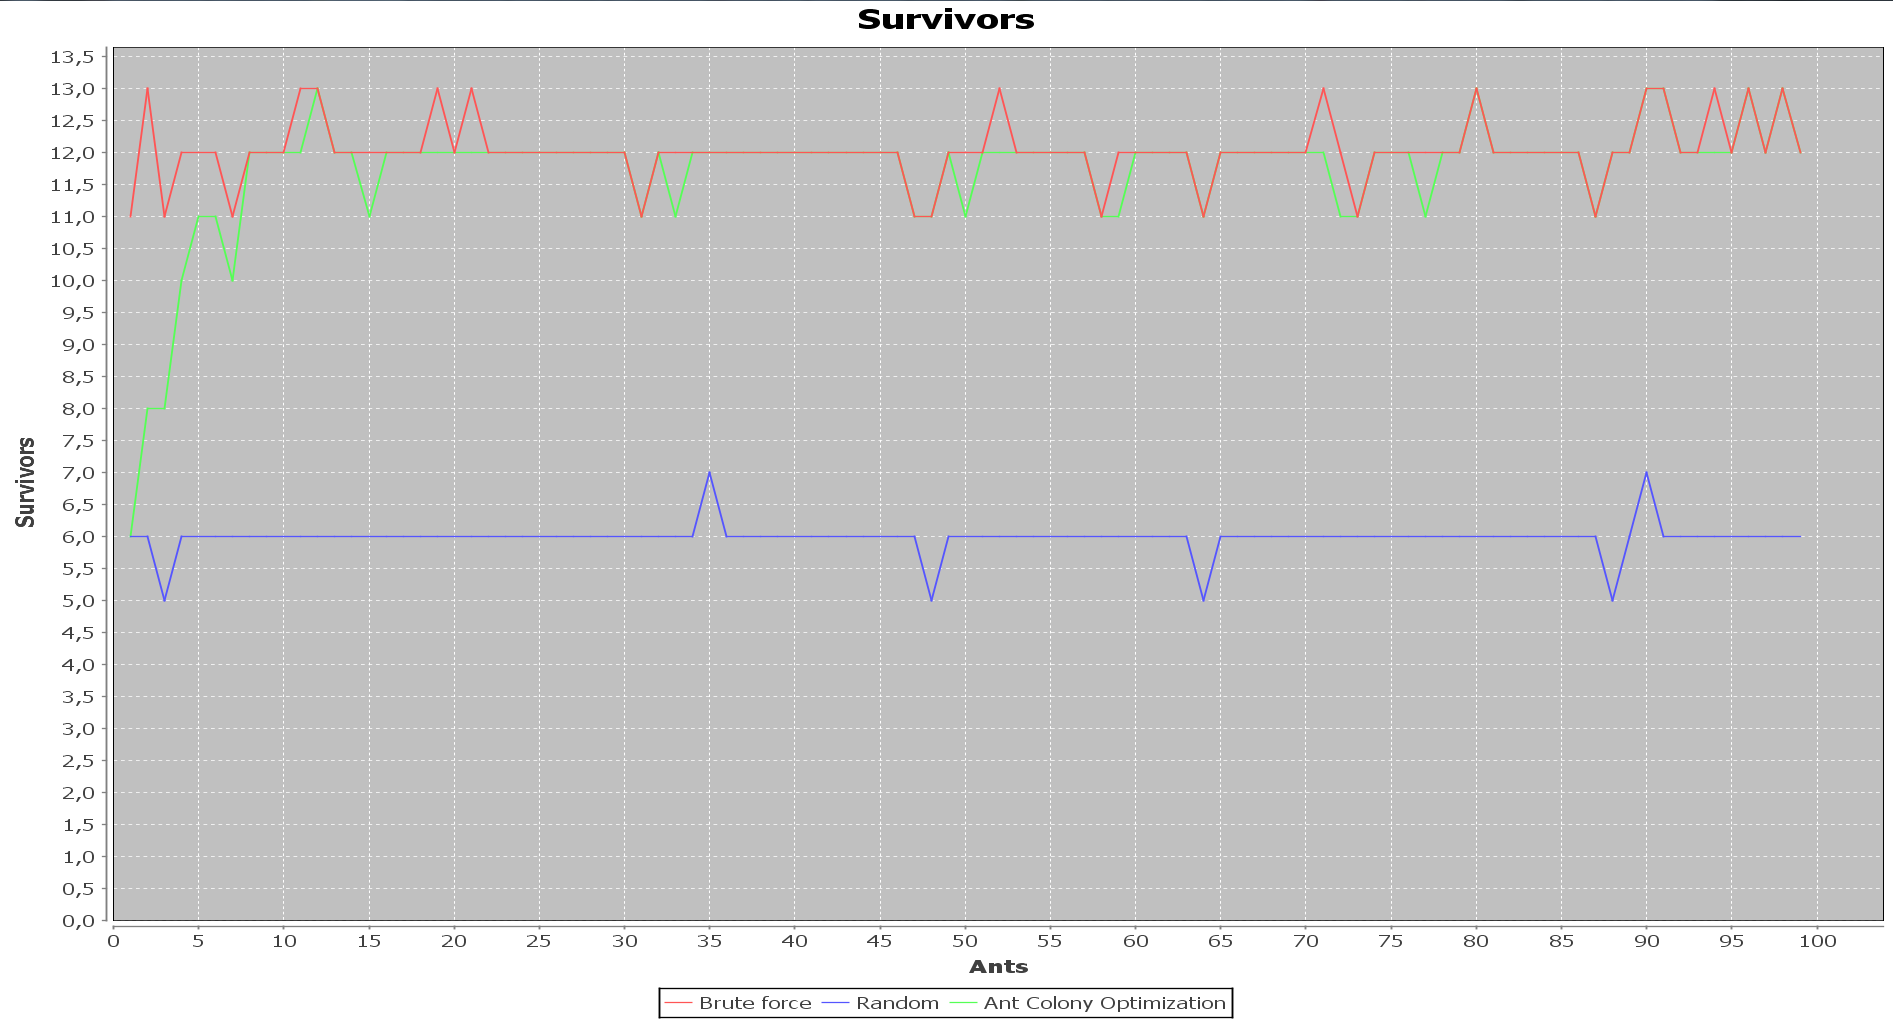
\includegraphics[width=160mm]{images/8Nodes2Leathal1Exit.png}
\caption{\textit{Graph with 8 nodes, where 2 are lethal and there is 1 exit.}}
\label{fig:Rsmallgraph}
\end{figure}


\begin{figure} % "placement and width parameter for the width of the image space.
\hspace*{-1.5 cm}
\includegraphics[width=160mm]{images/40Nodes2Leathal2Exit.png}
\caption{\textit{Graph with 40 nodes, where 2 are lethal and there is 1 exit.}}
\label{fig:Rbiggraph}
\end{figure}

\begin{figure} % "placement and width parameter for the width of the image space.
\hspace*{-1.5 cm}
\includegraphics[width=160mm]{images/Float8Nodes2Leathal1Exitpng.png}
\caption{\textit{Same as figure \ref{fig:Rsmallgraph}, however this is not absolute survivors.}}
\label{fig:Rsmallgraphf}
\end{figure}

The main difference from 8 to 40 nodes is that it requires more ants to solve the problem in bigger graphs, however it is not a huge increase. This can be shown in figure \ref{fig:Rsmallgraph} and figure \ref{fig:Rbiggraph}. There is also an increase of needed ants when more lethal nodes are added to the graph, in figure \ref{fig:Rbiggraph2f} ACO get close to brute force when ACO gets to use 20 ants or more, however when more lethal nodes are added shown in figure \ref{fig:Rbiggraph5f}, ACO needs more then 30 ants to get close to brute force, and is still not as good as ACO in figure \ref{fig:Rbiggraph2f}. This is to be expected as more lethal nodes makes more likely for the ants to stumble upon them.

\begin{figure} % "placement and width parameter for the width of the image space.
\hspace*{-1.5 cm}
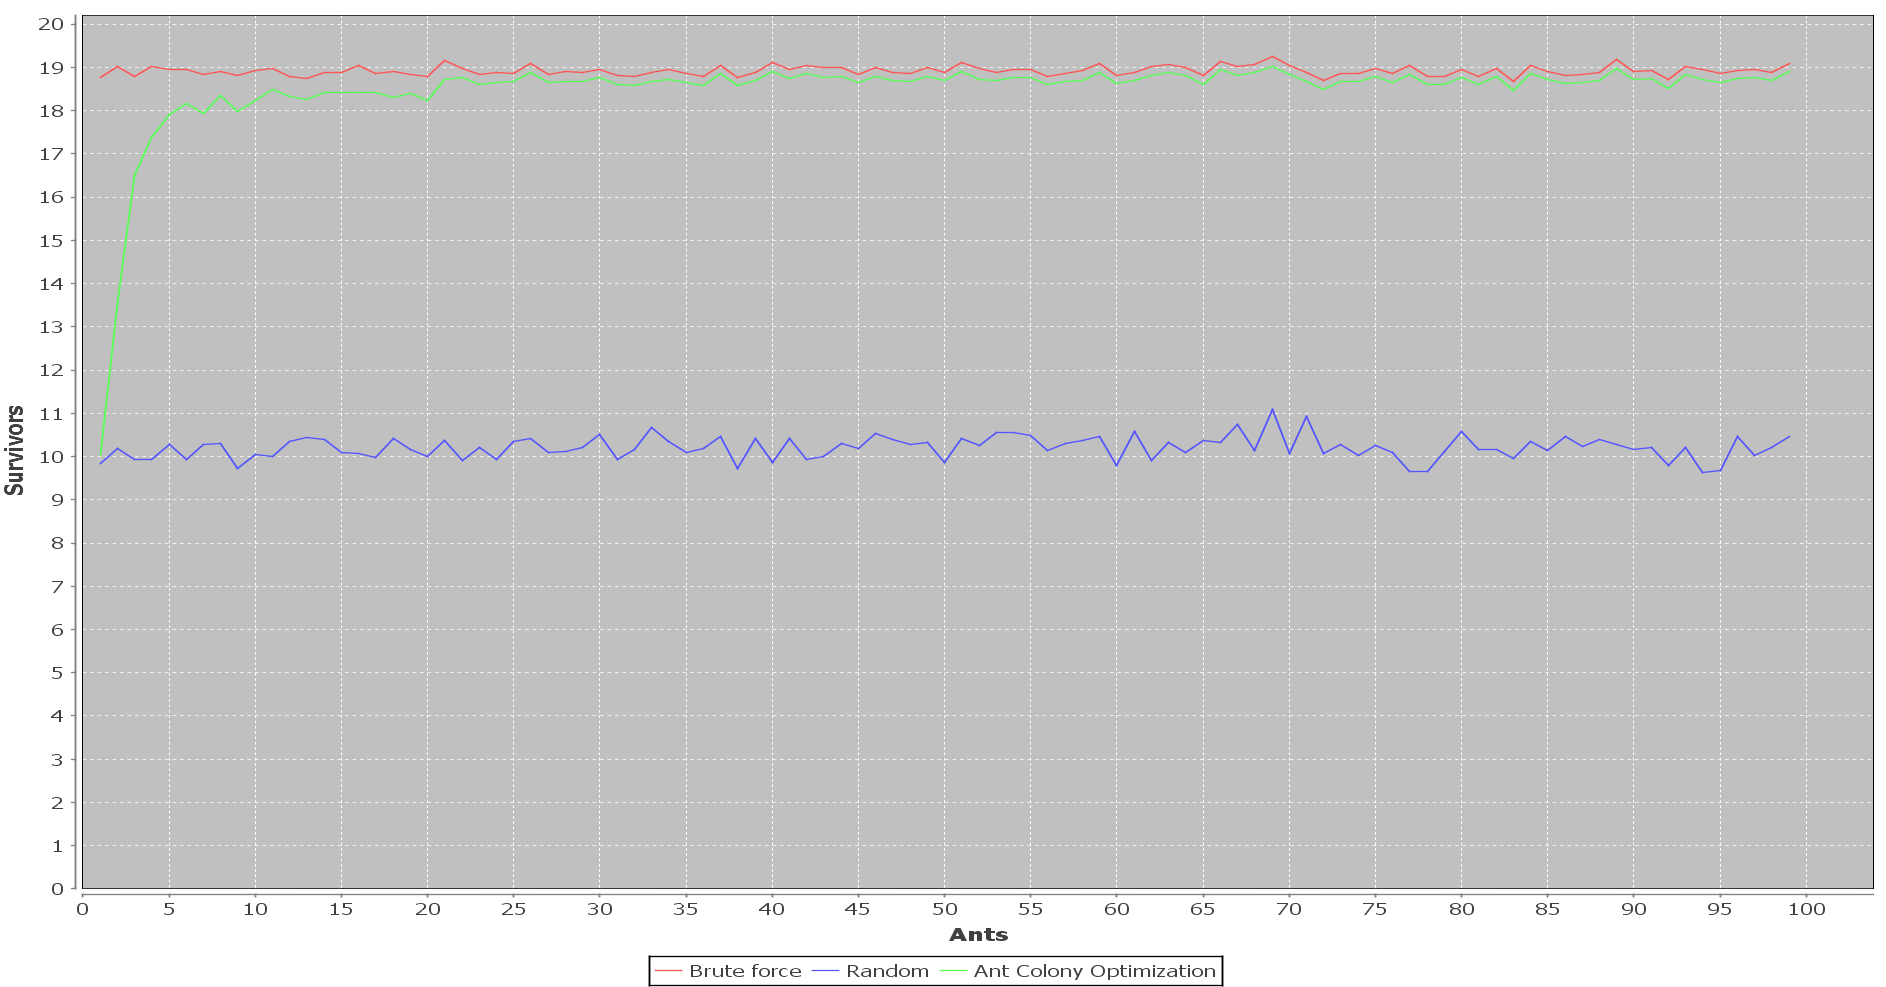
\includegraphics[width=160mm]{images/Float40Nodes2Leathal2Exit.png}
\caption{\textit{Same as figure \ref{fig:Rbiggraph}, however this is not absolute survivors.}}
\label{fig:Rbiggraph2f}
\end{figure}


\begin{figure} % "placement and width parameter for the width of the image space.
\hspace*{-1.5 cm}
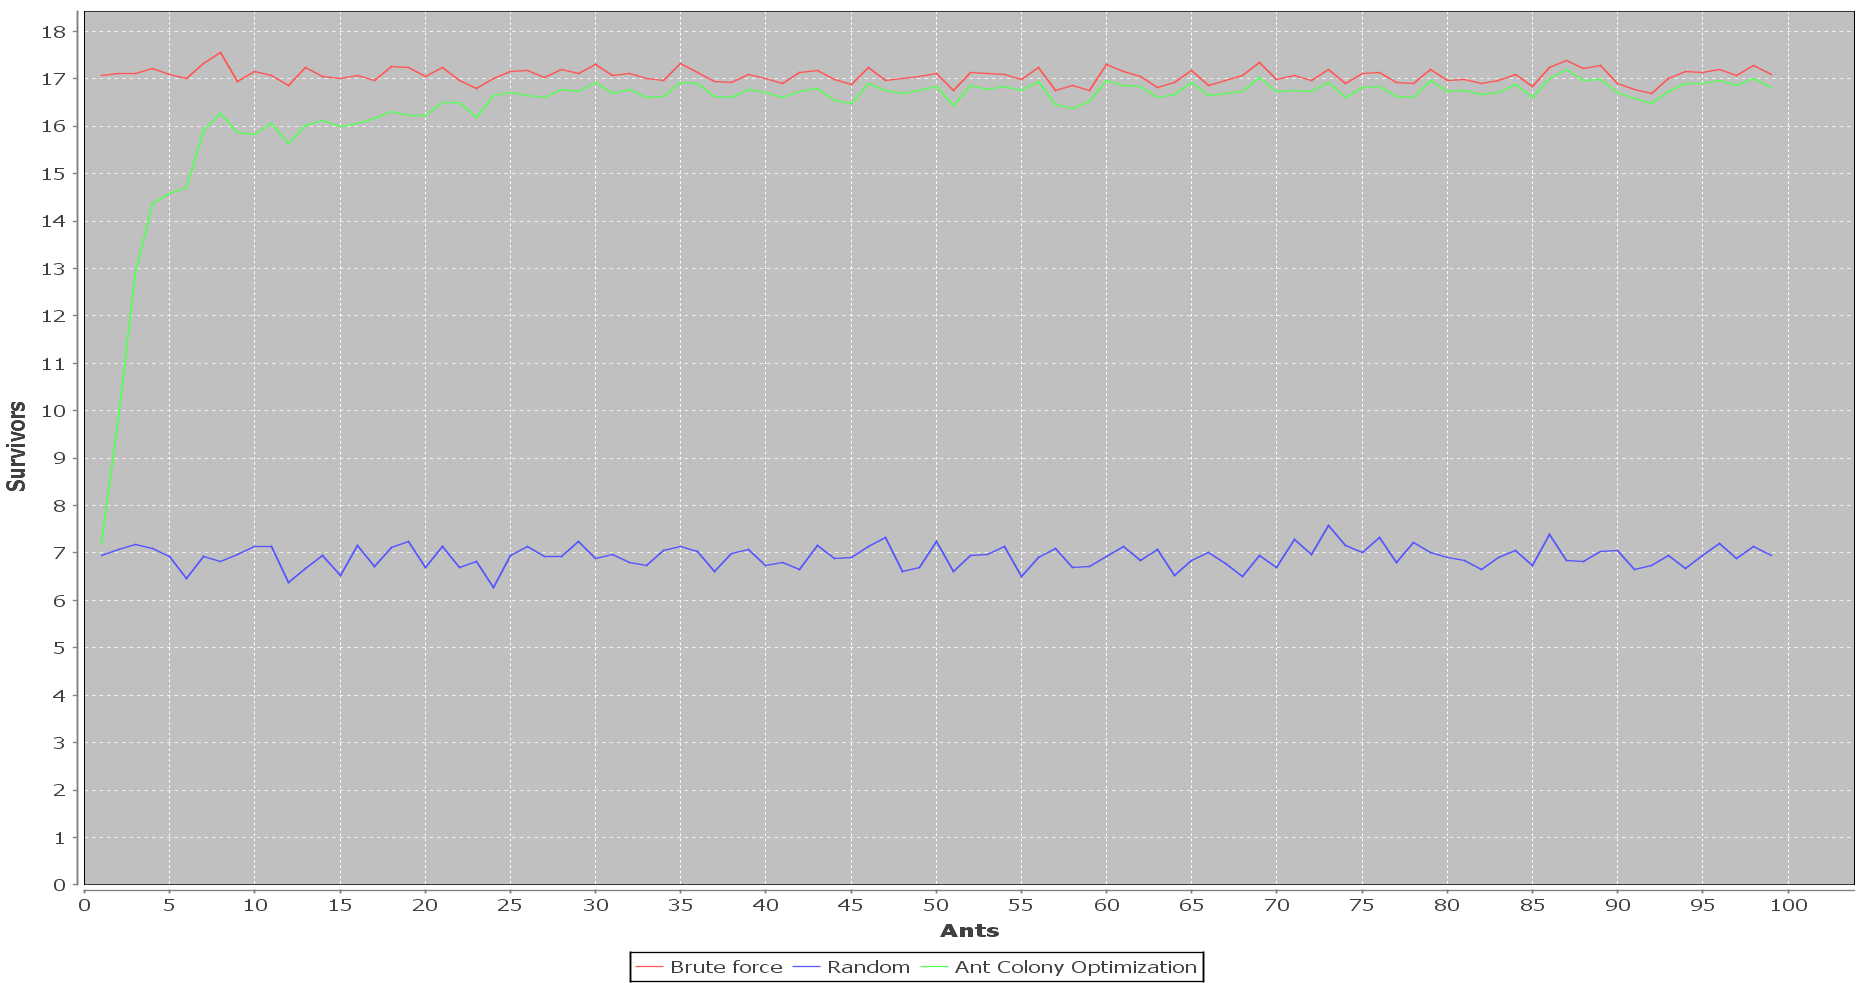
\includegraphics[width=160mm]{images/Float40Nodes5Leathal2Exit.png}
\caption{\textit{Same as figure \ref{fig:Rbiggraph2f}, only with 5 lethal nodes}}
\label{fig:Rbiggraph5f}
\end{figure}
\pagebreak

 Also, there is a difference when measuring absolute survivors and average survivors, in figure \ref{fig:Rsmallgraph} ACO reaches the same results as brute force, only to miss the target a few times, however in figure \ref{fig:Rsmallgraphf} ACO never reaches the exact same value, however is getting closer and closer as more ants are used in ACO.

ACO is not affected much by changing the lethal nodes after each turn, neither are random or brute force for that matter too. This is shown in the fact that they all ho up and down at at the same time. The only exception to this is when ACO only uses a few ants, as it gets better and better by using more ants to find solutions. This is a good thing as the next step is creating hazards that are dynamic and not stationary as this will be a bigger challenge for the AntSystem to solve. 





%\includegraphics[width=150mm]{Float8Nodes2Leathal1Exitpng.png}
%\includegraphics[width=150mm]{40Nodes2Leathal2Exit.png}
    \chapter{Conclusion and further work}
\label{ch:conclusion}
\textit{Approx. 5 pages}

\section{Summary of Results}

\section{Conclusion}
\emph{``My conclusion offers a compelling final comment to my argument, one that is persuasive for my
intended audience.''}

\section{Contributions}
List of contributions to new knowledge

\section{Further Work}

    \begin{singlespace}
        \bibliographystyle{IEEEtranS}
        %\bibliographystyle{plain}
				%\bibliographystyle{apalike}
        \bibliography{bib/web}
    \end{singlespace}

    \printglossary   

\end{document}

